\chapter{Marco teórico}\label{cap:marco}

Este capítulo reúne las herramientas que usa el trabajo. La sección~\ref{sec:altura} define cómo se mide la altura en
24-EDO y la estructura algebraica de sus clases. La sección~\ref{sec:senal} resume el procesamiento de señales que lleva
del audio a las alturas. La sección~\ref{sec:armonia-teoria} presenta la teoría armónica que se extiende a 24-EDO, y la
sección~\ref{sec:estadistica}, las medidas con que se comparan canciones y estilos.

\section{La altura en 24-EDO}\label{sec:altura}

\subsection{Escala logarítmica y cents}

La percepción de la altura es aproximadamente logarítmica en la frecuencia: subir una octava es multiplicar la frecuencia
por dos. Para medir distancias de manera lineal se usa el \emph{cent}.

\begin{definicion}[Cents]
La distancia en cents entre una frecuencia $f$ y una frecuencia de referencia $f_0$ es
\[
  c(f, f_0) = 1200 \log_2\!\left(\frac{f}{f_0}\right).
\]
Una octava mide 1200 cents y un semitono del temperamento de doce notas, 100.
\end{definicion}

\begin{definicion}[$q$-EDO]
En el sistema $q$-EDO (\emph{equal divisions of the octave}) la octava se divide en $q$ pasos iguales. Cada paso mide
$1200/q$ cents y corresponde a la razón de frecuencias
\[
  \rho_q = 2^{1/q}, \qquad f_j = f_{\mathrm{ref}}\, 2^{j/q}.
\]
\end{definicion}

Para $q = 12$ se obtiene el temperamento igual usual. Para $q = 24$ cada paso mide 50 cents, un cuarto de tono, y la razón
entre pasos consecutivos es $\alpha = 2^{1/24} \approx 1.0293$: cada traste del instrumento de la banda sube la frecuencia
cerca de un 2.93\,\%. Esta rejilla es la que forma las filas del tabroll.

\subsection{MIDI fraccionario y clases de altura}

El estándar MIDI numera las teclas del piano con enteros y asigna el número 69 al La de 440~Hz \citep{midi1996}. Su
extensión continua permite números fraccionarios:
\[
  M(f) = 69 + 12 \log_2\!\left(\frac{f}{440}\right).
\]
Así, el Mi de la nota 52 subido 50 cents queda en $M = 52.5$: un cuarto de tono sobre Mi, que un sistema de doce notas
redondearía a Mi o a Fa. La clase de altura en 24-EDO se obtiene redondeando al medio semitono y reduciendo módulo la
octava:
\[
  \operatorname{pc}_{24}(M) = \round(2M) \bmod 24 \in \mathbb{Z}_{24}.
\]
Una altura cae en una casilla de 24-EDO si está a menos de 25 cents de su centro. Las clases pares son los doce grados
regulares (Do, Do\sh, Re, \dots) y las impares, los doce grados en cuarto de tono, que se escriben con «+»: Do+, Re+,
etc. Los grados se cuentan desde la tónica de la canción; por ejemplo, \fl2+ es el segundo grado rebajado un semitono y
subido un cuarto de tono.

Contar los grados desde la tónica $t$ equivale a aplicar la transposición $T_{-t}$, con $T_k(y) = y + k$ en
$\mathbb{Z}_{24}$, así que los perfiles y los grados de este trabajo son los mismos en cualquier tonalidad. Las
transposiciones y las inversiones $I_n(y) = n - y$ forman juntas el grupo diédrico $D_{24}$, de 48 elementos: las simetrías
de un polígono de 24 lados \citep{crans2009,flynn2025}. La herramienta usa solo las transposiciones, a propósito: una
inversión convierte una tríada mayor en una menor ($I_0$ lleva Do mayor a fa menor), y esa diferencia es una de las que
se quieren medir.

\subsection{Los dos campos de quintas}\label{sec:campos}

En 24-EDO la quinta justa temperada mide 700 cents, es decir, 14 pasos de cuarto de tono. El ciclo de quintas es la
órbita de una clase bajo la suma reiterada de 14 en $\mathbb{Z}_{24}$.

\begin{proposicion}\label{prop:campos}
El subgrupo de $\mathbb{Z}_{24}$ generado por $14$ es $\langle 14 \rangle = \langle 2 \rangle = \{0, 2, 4, \dots, 22\}$,
de orden 12. En consecuencia, el ciclo de quintas de 24-EDO se parte en dos órbitas disjuntas de doce clases: los grados
regulares (clases pares) y los grados en cuarto de tono (clases impares).
\end{proposicion}

\begin{proof}
En un grupo cíclico $\mathbb{Z}_n$, el subgrupo generado por $a$ es el generado por $\mcd(a, n)$ y tiene orden
$n / \mcd(a, n)$. Como $\mcd(14, 24) = 2$, se tiene $\langle 14 \rangle = \langle 2 \rangle$, de orden $24/2 = 12$. Sus
dos clases laterales, $\langle 2 \rangle$ y $1 + \langle 2 \rangle$, son las clases pares e impares, y la suma de 14
conserva la paridad.
\end{proof}

Cada órbita se llama un \emph{campo}. Alois Hába armonizaba dentro de un solo campo y pasaba de uno al otro por la
melodía, lo que se ha llamado «desplazamiento de campos» \citep{little2019}. En su tratado, Hába describe la gama de
cuartos de tono como dos mitades, los doce grados convencionales y los doce en cuarto de tono, y para pasar de una a otra
recomienda movimiento contrario en las voces extremas \citep[cap.~II]{haba1927}; \citet[cap.~3]{skinner2006} encuentra en
su \emph{Suite für vier Posaunen}, op.~72, acordes puramente convencionales que alternan con acordes puramente en cuarto
de tono, aunque la regla del movimiento contrario no siempre se cumple. El manual de Wyschnegradsky deja ver por qué
funciona esa regla: dos escalas de cuartos de tono en movimiento contrario que parten del unísono dan, paso a paso, todos
los intervalos tradicionales \citep[§11, p.~6]{wyschnegradsky2017}. Cada voz cambia de campo en cada paso, pero las dos lo
hacen a la vez, así que nunca quedan en campos distintos. En las figuras del círculo de 24-EDO
(capítulo~\ref{cap:resultados}) el anillo exterior es el campo regular y el interior, el de cuarto de tono; cada grado
«+» queda junto a su vecino regular.

La misma imagen aparece en Ivan Wyschnegradsky. En su \emph{Manuel d'harmonie à quarts de ton} (1932) describe los doce
grados nuevos como la relación entre dos escalas cromáticas, una transportada un cuarto de tono, que se parecen a dos
peines cuyos dientes encajan \citep[§3, p.~1]{wyschnegradsky2017}. En el mismo manual observa que el ciclo de terceras
neutras recorre las 24 notas y se parte en dos ciclos de quintas, separados por una tercera neutra
\citep[§10, p.~5]{wyschnegradsky2017}. Es la proposición~\ref{prop:campos} vista desde la tercera neutra: como
$\mcd(7, 24) = 1$, sumar 7 recorre todo $\mathbb{Z}_{24}$, y sumar 7 dos veces es sumar 14, la quinta, que no sale del
campo. Charles Ives la llevó al instrumento en sus \emph{Three Quarter-Tone Pieces}
(1923--1924), para dos pianos afinados a un cuarto de tono de distancia \citep{ives1968}: un piano toca solo el campo
regular y el otro, solo el de cuarto de tono \citep{flynn2025}.

\begin{proposicion}\label{prop:z12}
La aplicación $\iota : \mathbb{Z}_{12} \to \mathbb{Z}_{24}$, $\iota(r) = 2r$, es un monomorfismo de grupos cuya imagen es
el campo regular $\langle 2 \rangle$. En consecuencia, todo análisis en doce notas se reproduce dentro de 24-EDO, y el
campo de cuarto de tono es la clase lateral $1 + \iota(\mathbb{Z}_{12})$, que ningún análisis en doce notas puede ver.
\end{proposicion}

\begin{proof}
$\iota(r + s) = 2(r + s) = \iota(r) + \iota(s)$ módulo 24, y $\iota(r) = 0$ en $\mathbb{Z}_{24}$ implica $24 \mid 2r$, es
decir, $12 \mid r$, de modo que $r = 0$ en $\mathbb{Z}_{12}$. La imagen tiene 12 elementos, todos pares, así que es
$\langle 2 \rangle$.
\end{proof}

\subsection{Razones justas y su aproximación en 24-EDO}

Los intervalos «naturales» de la serie armónica corresponden a razones de enteros pequeños: la octava $2/1$, la quinta
$3/2$, la tercera mayor $5/4$. Un sistema $q$-EDO aproxima cada razón $r$ por el paso más cercano.

\begin{proposicion}
Sea $c(r) = 1200 \log_2 r$ el tamaño en cents de la razón $r$. Su mejor aproximación en $q$-EDO,
$\hat c(r) = \tfrac{1200}{q} \round\!\bigl(\tfrac{q}{1200} c(r)\bigr)$, cumple $|c(r) - \hat c(r)| \le 600/q$. Además,
el error en 24-EDO nunca es mayor que el error en 12-EDO.
\end{proposicion}

\begin{proof}
La primera afirmación es la cota del redondeo al múltiplo más cercano de $1200/q$. Para la segunda, la rejilla de 12-EDO
está contenida en la de 24-EDO (proposición~\ref{prop:z12}), así que el punto más cercano en la rejilla fina está al
menos tan cerca como el más cercano en la gruesa.
\end{proof}

La tabla~\ref{tab:razones} muestra por qué 24-EDO no es solo «12-EDO con más notas»: aproxima intervalos de la serie
armónica que 12-EDO no tiene, como la tercera neutra $11/9$ y la segunda neutra $12/11$, presentes en el maqam árabe. Los nombres de los
intervalos nuevos son los de \citet[§6, pp.~2--3]{wyschnegradsky2017}: segunda, tercera, sexta y séptima neutras (3, 7,
17 y 21 cuartos de tono), a medio camino entre la menor y la mayor.

\begin{table}[ht]
  \centering
  \caption{Algunas razones justas y su aproximación en 12-EDO y en 24-EDO (en cents).}\label{tab:razones}
  \begin{tabular}{@{}llrrr@{}}
    \toprule
    Intervalo & Razón & Justo & 12-EDO (error) & 24-EDO (error) \\
    \midrule
    Quinta justa & $3/2$ & 702.0 & 700 ($-2.0$) & 700 ($-2.0$) \\
    Tercera mayor & $5/4$ & 386.3 & 400 ($+13.7$) & 400 ($+13.7$) \\
    Tercera menor & $6/5$ & 315.6 & 300 ($-15.6$) & 300 ($-15.6$) \\
    Tercera neutra & $11/9$ & 347.4 & 300 o 400 ($\pm 50$) & 350 ($+2.6$) \\
    Segunda neutra & $12/11$ & 150.6 & 100 o 200 ($\pm 50$) & 150 ($-0.6$) \\
    Cuarta del 11.º armónico & $11/8$ & 551.3 & 500 o 600 ($\pm 50$) & 550 ($-1.3$) \\
    \bottomrule
  \end{tabular}
\end{table}

\section{Microtonalidad, modos y looper}\label{sec:contexto-musical}

\subsection{Modos}

Un \emph{modo} es una escala de siete grados con un centro. Los modos que aparecen en este trabajo se distinguen por
los grados 2, 3, 6 y 7, medidos en semitonos sobre la tónica:

\begin{itemize}
  \item \textbf{Dórico:} 1, 2, \fl3, 4, 5, 6, \fl7. Es un menor con la sexta mayor; «So What» de Miles Davis, que la banda
  menciona, está en dórico.
  \item \textbf{Frigio:} 1, \fl2, \fl3, 4, 5, \fl6, \fl7. Es un menor con la segunda rebajada, de sonido «oriental» o
  «flamenco».
  \item \textbf{Frigio dominante:} 1, \fl2, 3, 4, 5, \fl6, \fl7. Es el frigio con la tercera mayor; entre \fl2 y 3 queda
  una segunda aumentada. Es la escala más cercana, en doce notas, al maqam hijaz.
  \item \textbf{Mixolidio:} 1, 2, 3, 4, 5, 6, \fl7. Es un mayor con la séptima rebajada, frecuente en el rock.
\end{itemize}

En 24-EDO cada uno de esos grados puede aparecer además en su versión neutra, un cuarto de tono por encima de la
rebajada, con el nombre que \citet[§6]{wyschnegradsky2017} da a esos intervalos: \fl2+, \fl3+, \fl6+ y \fl7+ son la
segunda, la tercera, la sexta y la séptima neutras. La herramienta no fuerza un nombre de doce notas: describe el modo por la versión de los grados 2, 3, 6 y 7 que
más suena (por ejemplo «\fl2+, 3, \fl6+, \fl7»).

\subsection{La microtonalidad en otras tradiciones}

\paragraph{Maqam árabe.} La teoría árabe del siglo XX describe sus escalas sobre una rejilla de 24 cuartos de tono \citep{touma1996},
aunque la afinación real de cada intervalo varía según el maqam y la región. Varios maqamat usan segundas y terceras
neutras (por ejemplo rast y bayati). Hijaz, el que menciona David Bennett, se caracteriza por la segunda aumentada entre
el segundo y el tercer grado, y en doce notas se parece al frigio dominante \citep{touma1996}.

\paragraph{Makam turco.} La teoría de Arel, Ezgi y Uzdilek divide el tono en nueve comas de Holder (la octava en 53
partes), lo que da intervalos que no caen en 24-EDO. Por eso SymbTr guarda las alturas en comas \citep{karaosmanoglu2012}
y los estudios de altura del makam usan histogramas finos \citep{bozkurt2008,gedik2010}.

\paragraph{Radif persa.} El radif es el repertorio clásico de la música persa, organizado en siete \emph{dastgah} y cinco
\emph{avaz} \citep{farhat1990}. La notación moderna usa dos alteraciones microtonales: el \emph{koron}, que baja una nota
aproximadamente un cuarto de tono, y el \emph{sori}, que la sube \citep{kanani2025}.

\paragraph{Alois Hába.} El compositor checo Alois Hába (1893--1973) escribió obras en cuartos, quintos y sextos de
tono, y en 1927 publicó la \emph{Neue Harmonielehre}, una teoría de la armonía para los sistemas de tercios, cuartos,
sextos y doceavos de tono \citep{haba1927,choroscian2018}. Su música en cuartos de tono se ha estudiado en los cuartetos
de cuerda \citep{choroscian2018}, en las obras para violín solo \citep{jin2015} y en la suite para cuatro trombones
\citep{skinner2006}; desde 1924 enseñó cuartos de tono en el Conservatorio de Praga y trabajó con la casa Förster en
pianos y armonios de cuarto y sexto de tono \citep{spurny2021}. Su idea de armonizar dentro de un campo y desplazarse
entre campos por la melodía es la que se pone a prueba en la sección~\ref{sec:res-haba}.

\paragraph{King Gizzard and the Lizard Wizard.} En \emph{Flying Microtonal Banana} (2017) la banda australiana usó
guitarras y bajos con trastes de cuarto de tono, es decir, el mismo 24-EDO que Angine de Poitrine; la nota de
lanzamiento del álbum termina con «24-TET EVERYBODY» \citep{kinggizzard2017}. Es el precedente más
cercano en el rock y por eso entra en la comparación (sección~\ref{sec:repertorios}).

\subsection{El looper}

Un looper es un dispositivo que graba una frase y la reproduce en bucle mientras el músico toca encima; cada nueva capa
se suma a las anteriores (\emph{overdub}). Una canción construida así tiene tres propiedades que el método aprovecha y
que, a la vez, lo dificultan:
\begin{enumerate}
  \item \textbf{Periodicidad:} dentro de una sección, el audio se repite con un periodo fijo, el largo del bucle. Esto
  permite promediar entre vueltas (sección~\ref{sec:met-consenso}).
  \item \textbf{Tempo constante:} el bucle no cambia de velocidad, de modo que la alineación con la partitura puede
  ajustarse a una recta por sección (sección~\ref{sec:evaluacion}).
  \item \textbf{Capas del mismo instrumento:} varias guitarras grabadas por la misma persona, con el mismo timbre, suenan a
  la vez. Ningún separador de fuentes las distingue, y ese es el cuello de botella de la melodía
  (sección~\ref{sec:res-separacion}).
\end{enumerate}

\section{Del audio a las alturas}\label{sec:senal}

\subsection{Transformada de Fourier de tiempo corto}

Un audio digital es una sucesión de amplitudes $x[n] = x(n/f_s)$, con $f_s$ la frecuencia de muestreo. Para saber qué
frecuencias suenan en cada instante, la señal se divide en ventanas y a cada una se le aplica la transformada discreta
de Fourier:
\begin{align*}
  X(m, k) &= \sum_{n=0}^{N-1} x[n + mH]\, w[n]\, e^{-2\pi i k n / N}, &
  f_k &= \frac{k f_s}{N},
\end{align*}
donde $w$ es la ventana, $N$ su tamaño y $H$ el salto entre ventanas. El espectrograma $S(m,k) = |X(m,k)|^2$ muestra
cómo cambia el contenido frecuencial en el tiempo. Una ventana larga mejora la resolución en frecuencia y empeora la
temporal; en este trabajo la ventana del análisis de altura es de 4096 muestras (186~ms a 22\,050~Hz), lo que hace que
las notas se detecten ligeramente antes de su ataque real (sección~\ref{sec:circulo-vivo}).

\subsection{Saliencia armónica}

Una nota de guitarra no es una sola frecuencia: tiene una fundamental $f$ y armónicos en $2f, 3f, \dots$. La
\emph{saliencia armónica} estima, para cada altura candidata $p$ y cada instante $t$, cuánta evidencia hay de que esa
altura suene, sumando la energía de sus armónicos con pesos decrecientes:
\[
  \Sigma(t, p) = \sum_{h=1}^{H} \beta^{\,h-1}\, \bigl| X\bigl(t,\, h f_p\bigr) \bigr|,
\]
con $H = 10$ armónicos, $\beta = 0.82$ y una altura candidata cada 25 cents, la mitad de un paso de 24-EDO. A diferencia
de un estimador de una sola voz, la saliencia mira todas las alturas a la vez, lo que permite seguir la melodía en una
textura polifónica \citep{salamon2012}.

\subsection{pYIN y el seguimiento de la altura}

pYIN \citep{mauch2014} estima la frecuencia fundamental de una sola voz buscando cada cuánto se repite la onda, a partir
del método YIN \citep{decheveigne2002}, y elige entre las lecturas posibles el camino más probable con un modelo oculto
de Markov. Funciona bien en una línea monofónica, pero entrega una sola altura por instante.

\subsection{El algoritmo de Viterbi}

El algoritmo de Viterbi \citep{viterbi1967} encuentra, en una sucesión de estados con puntajes locales y costos de
transición, la sucesión de puntaje máximo. Sea $\{1, \dots, N\}$ el conjunto de estados (las alturas candidatas), $e_t(j)$
el puntaje de estar en el estado $j$ en el instante $t$ y $c(i, j) \ge 0$ el costo de pasar de $i$ a $j$. El puntaje de un
camino $x = (x_1, \dots, x_T)$ es
\[
  J(x) = \sum_{t=1}^{T} e_t(x_t) - \sum_{t=2}^{T} c(x_{t-1}, x_t).
\]

\begin{proposicion}[Principio de optimalidad]\label{prop:viterbi}
Sea $\delta_1(j) = e_1(j)$ y, para $t \ge 2$,
\[
  \delta_t(j) = e_t(j) + \max_{i} \bigl[\delta_{t-1}(i) - c(i, j)\bigr].
\]
Entonces $\delta_t(j)$ es el máximo de $J$ sobre los caminos de longitud $t$ que terminan en $j$, y
$\max_x J(x) = \max_j \delta_T(j)$. El camino óptimo se recupera guardando en cada paso el $i$ que realiza el máximo.
\end{proposicion}

\begin{proof}
Por inducción en $t$. Para $t = 1$ es la definición. Si la afirmación vale en $t - 1$, todo camino de longitud $t$ que
termina en $j$ se escribe como un camino de longitud $t - 1$ que termina en algún $i$, seguido del paso $i \to j$. Su
puntaje es el del prefijo más $e_t(j) - c(i, j)$. Para $i$ fijo, el mejor prefijo vale $\delta_{t-1}(i)$ por hipótesis de
inducción, así que el máximo sobre todos los caminos es $e_t(j) + \max_i [\delta_{t-1}(i) - c(i,j)] = \delta_t(j)$.
\end{proof}

El cálculo cuesta $O(T N^2)$ operaciones, o $O(T N W)$ si los saltos se limitan a $W$ estados. En este trabajo los
estados son las alturas candidatas cada 25 cents más un estado «sin altura»; el puntaje local es
$e_t(j) = \log\bigl(1 + \Sigma(t, p_j)/\theta\bigr)$, con $\theta$ el percentil 55 de la saliencia máxima; el costo de
transición es $c(i, j) = 0.01\, |i - j|$ (0.01 por paso de 25 cents, con saltos de hasta 96 pasos), y entrar o salir del
estado sin altura cuesta 1. El contorno resultante sigue la altura con más evidencia sin dar saltos innecesarios.

\subsection{Pulso y compases por programación dinámica}

El mismo principio sirve para el ritmo. \citet{ellis2007} plantea el seguimiento del pulso como la búsqueda de una
sucesión de instantes $t_1 < t_2 < \dots$ que caigan sobre ataques fuertes y estén separados aproximadamente por el
periodo $\tau_0$ del tempo:
\[
  C(t) = o(t) + \max_{\tau \in [\tau_0/2,\, 2\tau_0]} \Bigl[ C(t - \tau) - \alpha \log^2\!\bigl(\tau/\tau_0\bigr) \Bigr],
\]
donde $o(t)$ es la envolvente de ataques y $\alpha$ controla qué tan rígido es el tempo. Por la
proposición~\ref{prop:viterbi}, el máximo de $C$ se obtiene en una pasada y los pulsos se recuperan hacia atrás. La
división en compases se resuelve igual, sobre la sucesión de pulsos (sección~\ref{sec:met-compases}).

\subsection{Timbre: escala Mel y MFCC}

La escala Mel aproxima cómo agrupa el oído las frecuencias \citep{stevens1937}:
$\operatorname{mel}(f) = 2595 \log_{10}(1 + f/700)$. Un banco de filtros triangulares en esa escala resume el
espectrograma en bandas, y la transformada coseno discreta del logaritmo de sus energías da los coeficientes cepstrales
en escala Mel (MFCC) \citep{davis1980}. Los MFCC describen el timbre, no la nota; en este trabajo solo se usaron en el
primer algoritmo (sección~\ref{sec:primer-algoritmo}).

\section{Teoría armónica extendida a 24-EDO}\label{sec:armonia-teoria}

\subsection{Calidades de acorde según Piston}

\citet{piston1987} clasifica los acordes por sus intervalos sobre la fundamental. En 24-EDO aparece una calidad que no
existe en doce notas: la tríada con \emph{tercera neutra}, a 350 cents, justo entre la menor y la mayor. Wyschnegradsky
la llama \emph{neutral fifth chord} y la describe como dos terceras neutras superpuestas, entre el acorde mayor y el
menor, y simétrica como el aumentado y el disminuido
\citep[§16, p.~8]{wyschnegradsky2017}. La
tabla~\ref{tab:calidades} muestra las ocho calidades que usa la herramienta.

\begin{table}[ht]
  \centering
  \caption{Calidades de acorde de Piston extendidas a 24-EDO.}\label{tab:calidades}
  \begin{tabular}{llc}
    \toprule
    Calidad & Tercera (o intervalo característico) & Pasos de \cuarto{} de tono \\
    \midrule
    5 (quinta sola) & — & — \\
    m (menor) & 3.ª menor, 300 cents & 6 \\
    \textbf{n (neutra)} & \textbf{3.ª neutra, 350 cents} & \textbf{7} \\
    M (mayor) & 3.ª mayor, 400 cents & 8 \\
    disminuida · aumentada & 3.ª menor · 3.ª mayor & 6 · 8 \\
    sus2 · sus4 & 2.ª · 4.ª & 4 · 10 \\
    \bottomrule
  \end{tabular}
\end{table}

Piston distingue además grados tonales (I, IV, V), casi tonal (II) y modales (III y VI), y propone una medida del centro
en tres partes para música sin dominante, que este trabajo adapta (sección~\ref{sec:armonia-metodo}). Piston deja fuera
las escalas microtonales \citep[p.~474]{piston1987}; por eso, en este trabajo, los grados en cuarto de tono reciben una
función \emph{neutra}.

\subsection{Tríadas, transformaciones y campos}\label{sec:triadas-campos}

Con fundamental $x \in \mathbb{Z}_{24}$, las tríadas mayor, menor y neutra son $\{x, x+8, x+14\}$, $\{x, x+6, x+14\}$ y
$\{x, x+7, x+14\}$ \citep{flynn2025}.

\begin{proposicion}\label{prop:neutra}
Las tríadas mayor y menor tienen sus tres notas en un mismo campo, el de su fundamental. La tríada neutra tiene siempre
notas en los dos campos: la fundamental y la quinta en el campo de $x$, y la tercera neutra en el otro.
\end{proposicion}

\begin{proof}
Los intervalos 6, 8 y 14 son pares, así que $x+6$, $x+8$ y $x+14$ tienen la paridad de $x$. El 7 es impar, así que $x+7$
tiene la paridad contraria.
\end{proof}

Por eso un acorde con tercera neutra es, por construcción, una mezcla vertical de campos en el sentido de la
sección~\ref{sec:res-haba}: no se puede tocar sin una nota de cada campo.

En la teoría neorriemanniana, las transformaciones $P$ (paralela: Do mayor $\to$ do menor), $R$ (relativa: Do mayor $\to$
la menor) y $L$ (intercambio de sensible: Do mayor $\to$ mi menor) cambian una sola nota de la tríada y conservan las
otras dos. Cada una es una inversión $I_n$ cuyo eje pasa entre las dos notas que se conservan, es decir, $n$ es la suma de
esas dos notas \citep{crans2009}. \citet{flynn2025} las llevan a 24-EDO y muestran que, sobre las tríadas mayores y
menores, actúan por separado en cada campo, como dos copias del grupo de doce notas. La razón es de paridad.

\begin{proposicion}\label{prop:plr}
Si $X$ es una tríada mayor o menor, $P(X)$, $L(X)$ y $R(X)$ tienen su fundamental en el mismo campo que $X$, y entre
tríadas mayores y menores solo una transposición $T_k$ con $k$ impar cambia de campo. Sobre una tríada neutra, en
cambio, $P$ la deja igual y $L$ y $R$ siempre cambian de campo.
\end{proposicion}

\begin{proof}
Por la proposición~\ref{prop:neutra}, las tres notas de una tríada mayor o menor tienen la misma paridad; la suma $n$ de
dos de ellas es par, e $I_n(y) = n - y$ conserva la paridad de $y$. $T_k$ conserva la paridad si y solo si $k$ es par. En
la tríada neutra, $P$ conserva la fundamental y la quinta: $n = 2x + 14$ las intercambia y deja fija la tercera $x + 7$,
así que la tríada no cambia. $L$ y $R$ conservan la tercera neutra y una nota del campo de $x$, así que $n$ es impar e
$I_n$ cambia la paridad de cada nota.
\end{proof}

Lo que hace $P$ con la tríada neutra es la simetría que señala Wyschnegradsky: la inversión que intercambia la fundamental
y la quinta deja el acorde igual, como pasa con el aumentado y el disminuido.

\subsection{Funciones de Riemann}

\citet{riemann1893} agrupa los acordes en tres funciones: \emph{tónica}, el reposo; \emph{subdominante}, el
alejamiento; y \emph{dominante}, la tensión que pide volver. La herramienta asigna a cada grado una función con criterios
explícitos: \fl III, III y VI son tónica relativa; \fl VII es dominante modal (subtónica, sin sensible); II mayor es
dominante de la dominante; \fl II es la napolitana; \fl VI, la mixtura; y \sh IV, el tritono, queda sin función.

\subsection{Ejes de Lendvai}

\citet{lendvai1971}, en su análisis de Bartók, agrupa las doce clases por terceras menores en tres ejes. Medido en
semitonos sobre el centro, el eje de un grado es el grado módulo 3. Cada eje tiene una rama principal (polo y contrapolo,
a un tritono) y una secundaria; un polo puede reemplazar a su contrapolo sin cambiar de función
(tabla~\ref{tab:ejes}).

\begin{table}[ht]
  \centering
  \caption{Ejes de Lendvai sobre el centro tonal.}\label{tab:ejes}
  \begin{tabular}{lll}
    \toprule
    Eje & Rama principal (polo, contrapolo) & Rama secundaria \\
    \midrule
    Tónica & I, \sh IV & VI, \fl III \\
    Subdominante & IV, VII & II, \fl VI \\
    Dominante & V, \fl II & III, \fl VII \\
    \bottomrule
  \end{tabular}
\end{table}

En lenguaje de grupos, los tres ejes son las clases laterales del subgrupo $\langle 3 \rangle = \{0, 3, 6, 9\}$ de
$\mathbb{Z}_{12}$ (las terceras menores sobre el centro): $\langle 3 \rangle$, $1 + \langle 3 \rangle$ y
$2 + \langle 3 \rangle$. Con el centro en 0, la clase $\langle 3 \rangle = \{\mathrm{I}, \fl\mathrm{III}, \sh\mathrm{IV},
\mathrm{VI}\}$ es el eje de tónica; $1 + \langle 3 \rangle = \{\fl\mathrm{II}, \mathrm{III}, \mathrm{V}, \fl\mathrm{VII}\}$,
el de dominante; y $2 + \langle 3 \rangle = \{\mathrm{II}, \mathrm{IV}, \fl\mathrm{VI}, \mathrm{VII}\}$, el de
subdominante.

\paragraph{Extensión a 24-EDO (propuesta de este trabajo).} Un grado en cuarto de tono cae entre dos ejes vecinos.

\begin{proposicion}
La tercera menor mide 6 pasos de cuarto de tono, y el subgrupo $\langle 6 \rangle = \{0, 6, 12, 18\}$ de $\mathbb{Z}_{24}$
tiene seis clases laterales. Tres de ellas están contenidas en el campo regular $\langle 2 \rangle$ y son la imagen, por
$\iota$, de los tres ejes de Lendvai; las otras tres están en el campo de cuarto de tono y forman tres ejes nuevos, a los
que este trabajo llama \emph{ejes neutros}.
\end{proposicion}

\begin{proof}
$|\mathbb{Z}_{24} : \langle 6 \rangle| = 24/4 = 6$. Como $6$ es par, cada clase lateral $a + \langle 6 \rangle$ tiene todos
sus elementos con la paridad de $a$; las de $a = 0, 2, 4$ son pares y las de $a = 1, 3, 5$, impares. Además
$\iota(\langle 3 \rangle) = \langle 6 \rangle$ y $\iota(b + \langle 3 \rangle) = 2b + \langle 6 \rangle$, así que las tres
clases pares son las imágenes de los ejes de doce notas.
\end{proof}

Cada eje neutro queda entre dos ejes de Lendvai: T--D (1+, \fl3+, \sh4+, 6+), D--S (\fl2+, 3+, 5+, \fl7+) y S--T (2+, 4+,
\fl6+, 7+). El eje y la función de Riemann solo difieren en cuatro grados: III y \fl II son dominante para Lendvai, VII es
subdominante y \sh IV es tónica.

\section{Medidas de comparación}\label{sec:estadistica}

\subsection{Perfiles de 24 clases}

Una canción, o un compás, se resume en un perfil que dice qué fracción del tiempo suena cada clase. Si la nota $j$ ocupa
el intervalo $[a_j, b_j)$ y cae en la clase $r$,
\[
  h_r = \sum_{j:\, \operatorname{pc}_{24}(j) = r} (b_j - a_j), \qquad
  v_r = \frac{h_r}{\sum_{s=0}^{23} h_s}, \qquad v \in \mathbb{R}^{24},\ v_r \ge 0,\ \textstyle\sum_r v_r = 1.
\]
El mismo procedimiento, aplicado a las fundamentales de los acordes por compás y contado desde la tónica, da el
\emph{reparto de fundamentales} de una canción.

Los corpus de estilos están en doce notas, así que hay que llevar los perfiles de 24 clases a 12. Se usan dos
proyecciones, según el bloque:
\begin{itemize}
  \item En la armonía, la fundamental en cuarto de tono se lleva al grado de abajo, y la fracción de tiempo en que eso
  ocurre se informa aparte (columna «¼\,\%» de la matriz).
  \item En la escala, cada cuarto de tono se reparte mitad y mitad entre sus dos vecinos:
  $v^{(12)}_r = v_{2r} + \tfrac12 v_{2r-1} + \tfrac12 v_{2r+1}$, con índices módulo 24.
\end{itemize}

\subsection{Divergencias de Kullback-Leibler y de Jensen-Shannon}

La divergencia de Kullback-Leibler entre dos distribuciones $P$ y $Q$ es
\[
  D_{\mathrm{KL}}(P \,\|\, Q) = \sum_i P_i \log_2 \frac{P_i}{Q_i}.
\]
No es simétrica y puede ser infinita si $Q_i = 0$; por
eso se usa la divergencia de Jensen-Shannon \citep{lin1991}:
\[
  D_{\mathrm{JS}}(P, Q) = \tfrac12 D_{\mathrm{KL}}(P \,\|\, M) + \tfrac12 D_{\mathrm{KL}}(Q \,\|\, M),
  \qquad M = \tfrac12 (P + Q).
\]
Con logaritmos en base 2, $0 \le D_{\mathrm{JS}} \le 1$: vale 0 si las distribuciones coinciden y 1 si no comparten
masa. Su raíz cuadrada es una métrica. Por ejemplo, el reparto de fundamentales de «My Name Is Mud» (Primus) queda a
0.15 del centro del rock (figura~\ref{fig:formulas}).

\begin{figure}[htbp]
  \centering
  \begin{subfigure}{0.48\textwidth}\centering
    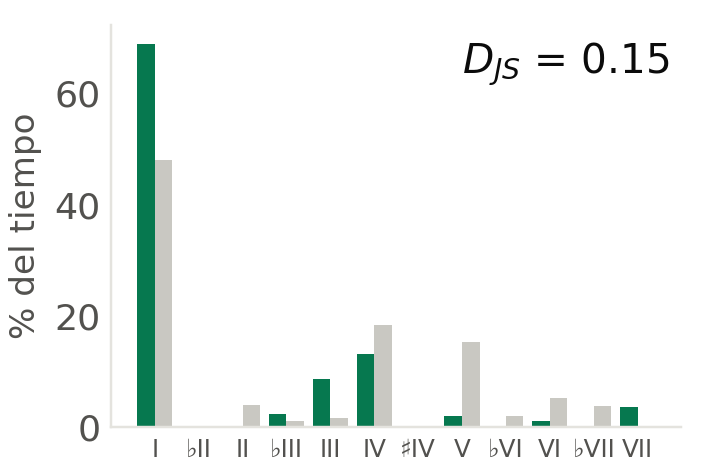
\includegraphics[width=\linewidth]{formula_js.png}
    \caption{Jensen-Shannon. Verde: fundamentales de «My Name Is Mud»; gris: centro del rock ($D_{\mathrm{JS}}=0.15$).}
  \end{subfigure}\hfill
  \begin{subfigure}{0.48\textwidth}\centering
    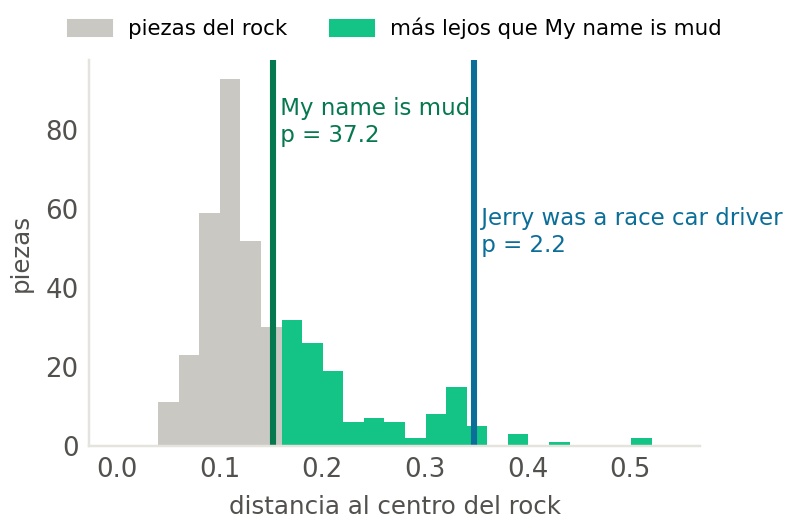
\includegraphics[width=\linewidth]{formula_percentil.png}
    \caption{Percentil. Gris: distancias de las piezas de rock a su centro; verde: las más lejanas que «My Name Is Mud» ($p=37.2$).}
  \end{subfigure}\\[0.8em]
  \begin{subfigure}{0.48\textwidth}\centering
    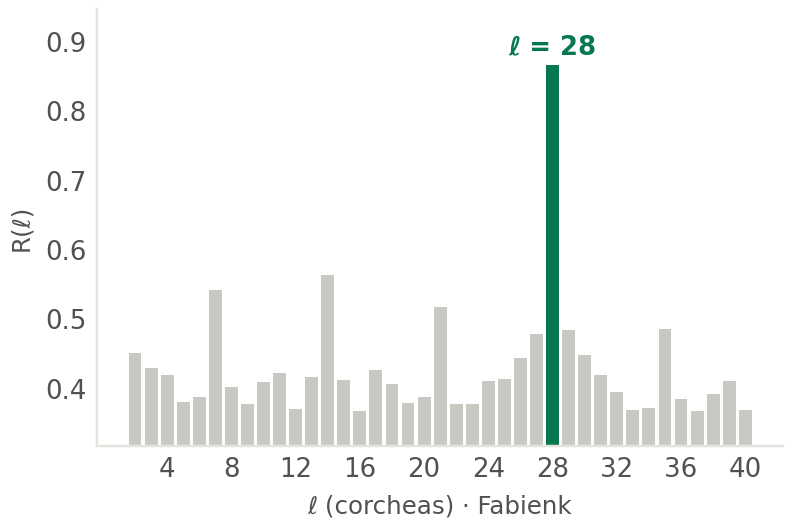
\includegraphics[width=\linewidth]{formula_repeticion.png}
    \caption{Repetición: $R(\ell)$ de «Jerry Was a Race Car Driver»; el pico en 8 corcheas es un compás de 4/4.}
  \end{subfigure}\hfill
  \begin{subfigure}{0.48\textwidth}\centering
    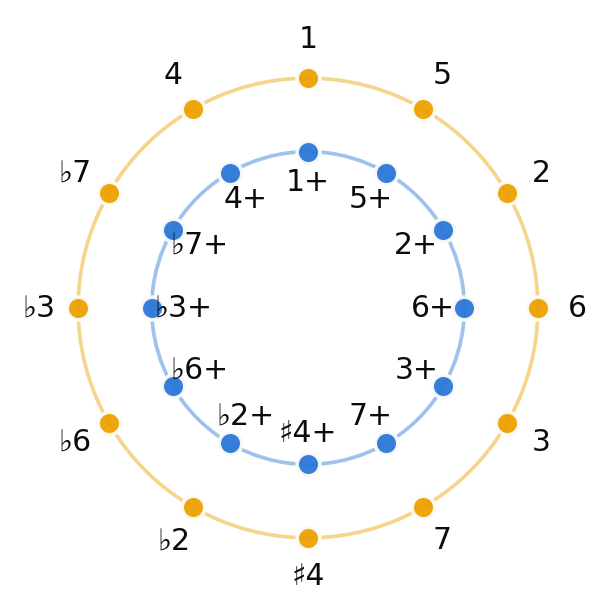
\includegraphics[width=\linewidth]{formula_campos.png}
    \caption{Los dos campos de quintas de 24-EDO: amarillo, el regular; azul, el de cuarto de tono.}
  \end{subfigure}
  \caption{Las medidas de comparación, ilustradas con canciones de Primus.}\label{fig:formulas}
\end{figure}

Las propiedades anteriores se deducen de la entropía de Shannon, $H(P) = -\sum_i P_i \log_2 P_i$ (con $0 \log 0 = 0$),
que mide en bits qué tan repartida está una distribución.

\begin{proposicion}[Desigualdad de Gibbs]
Para dos distribuciones $P$ y $Q$ sobre el mismo conjunto finito, $D_{\mathrm{KL}}(P \,\|\, Q) \ge 0$, con igualdad si y
solo si $P = Q$.
\end{proposicion}

\begin{proof}
Sea $I = \{i : P_i > 0\}$. Como $\log_2$ es cóncava, la desigualdad de Jensen da
\[
  -D_{\mathrm{KL}}(P \,\|\, Q) = \sum_{i \in I} P_i \log_2 \frac{Q_i}{P_i}
  \le \log_2 \sum_{i \in I} P_i \frac{Q_i}{P_i} = \log_2 \sum_{i \in I} Q_i \le \log_2 1 = 0.
\]
La igualdad en Jensen exige que $Q_i / P_i$ sea constante en $I$, y la segunda, que $\sum_{i \in I} Q_i = 1$; juntas
implican $P = Q$.
\end{proof}

\begin{proposicion}[Propiedades de Jensen-Shannon]\label{prop:js}
Para todo par de distribuciones $P, Q$:
\begin{enumerate}
  \item $D_{\mathrm{JS}}(P, Q) = H(M) - \tfrac12 H(P) - \tfrac12 H(Q)$, con $M = \tfrac12 (P + Q)$;
  \item $D_{\mathrm{JS}}(P, Q) = D_{\mathrm{JS}}(Q, P)$, y $D_{\mathrm{JS}}(P, Q) = 0$ si y solo si $P = Q$;
  \item $0 \le D_{\mathrm{JS}}(P, Q) \le 1$, y vale 1 si y solo si $P$ y $Q$ tienen soportes disjuntos;
  \item $D_{\mathrm{JS}}$ siempre es finita, aunque $P$ o $Q$ tengan ceros.
\end{enumerate}
\end{proposicion}

\begin{proof}
(1) Desarrollando, $D_{\mathrm{KL}}(P \,\|\, M) = -H(P) - \sum_i P_i \log_2 M_i$, y lo mismo para $Q$. Al promediar, los
términos cruzados suman $-\sum_i M_i \log_2 M_i = H(M)$.
(2) La simetría es evidente en la definición. Por Gibbs, cada sumando es no negativo y se anula solo si $P = M$ y
$Q = M$, es decir, si $P = Q$.
(3) Como $M_i \ge \tfrac12 P_i$, se tiene $\log_2 (P_i / M_i) \le \log_2 2 = 1$, así que
$D_{\mathrm{KL}}(P \,\|\, M) \le \sum_i P_i = 1$, y lo mismo para $Q$; el promedio es a lo sumo 1. La igualdad exige
$M_i = \tfrac12 P_i$ siempre que $P_i > 0$, es decir, $Q_i = 0$ donde $P_i > 0$, y viceversa.
(4) Si $P_i > 0$ entonces $M_i > 0$, de modo que ningún cociente $P_i / M_i$ se indefine.
\end{proof}

Que $\sqrt{D_{\mathrm{JS}}}$ satisfaga además la desigualdad triangular, y sea por tanto una métrica, es un resultado
más delicado \citep{endres2003}; en este trabajo se usa solo para justificar que las distancias entre canciones se pueden
comparar de manera coherente.

\subsection{Percentil de tipicidad}

Una distancia sola no dice si una canción es normal dentro de un estilo. El \emph{percentil de tipicidad} la compara con
las distancias de las propias piezas del corpus.

\begin{definicion}[Percentil de tipicidad respecto del centro]
Sea $C$ un corpus, $c$ su centro (el reparto promedio) y $d(x) = D_{\mathrm{JS}}(x, c_{-x})$ la distancia de cada pieza
al centro de las demás. Para una canción $s$,
\[
  p(s) = 100 \cdot \frac{\#\{x \in C : d(x) \ge d(s)\}}{|C|}.
\]
\end{definicion}

Un valor de 50 corresponde a una pieza típica del estilo; 0, a una canción más rara que todas las piezas del corpus.
«My Name Is Mud» da 37 en el rock y «Jerry Was a Race Car Driver», 2.2. Esta versión se usa en la matriz de armonía.

Un estilo puede tener varias zonas: un corpus con 93\,\% de piezas en 4 y 7\,\% en 3 tiene un promedio «en 4 con un poco
de 3» que no se parece a ninguna pieza. Por eso, en el test por bloques, la tipicidad se mide con vecinos.

\begin{definicion}[Percentil de tipicidad por vecinos]
Sea $d_k(s)$ la distancia de $s$ a su $k$-ésima pieza más cercana del corpus ($k = 5$). Para cada pieza $x \in C$ se
calcula $d_k(x)$ sin contarse a sí misma (ni a otra versión de la misma canción). Entonces
\[
  p_k(s) = 100 \cdot \frac{\#\{x \in C : d_k(x) \ge d_k(s)\}}{|C|}.
\]
\end{definicion}

\subsection{Percentil y significancia}

El percentil de tipicidad se puede leer como un valor $p$ empírico, y eso justifica el umbral de 5 que usa el veredicto.

\begin{proposicion}\label{prop:percentil}
Sea $C = \{x_1, \dots, x_n\}$ un corpus y $s$ una pieza nueva. Si $d(s), d(x_1), \dots, d(x_n)$ son intercambiables (por
ejemplo, si $s$ y las piezas del corpus provienen del mismo estilo) y no hay empates, entonces, para todo $u \in [0, 100]$,
\[
  \Pr\bigl[p(s) \le u\bigr] \le \frac{\lfloor u n / 100 \rfloor + 1}{n + 1} \approx \frac{u}{100}.
\]
\end{proposicion}

\begin{proof}
Por intercambiabilidad, el rango de $d(s)$ entre los $n + 1$ valores es uniforme en $\{1, \dots, n+1\}$. El percentil
$p(s)$ es $100/n$ veces el número de piezas del corpus con distancia mayor o igual; $p(s) \le u$ equivale a que a lo sumo
$\lfloor u n / 100 \rfloor$ piezas superen a $s$, es decir, a que $d(s)$ esté entre los $\lfloor u n / 100 \rfloor + 1$
valores más grandes. Esa probabilidad es $(\lfloor u n/100 \rfloor + 1)/(n + 1)$.
\end{proof}

En palabras: una pieza auténtica del estilo cae por debajo del percentil 5 alrededor del 5\,\% de las veces. Por eso el
umbral $u = 5$ funciona como un contraste a una cola con nivel 5\,\%, y la calibración del capítulo~\ref{cap:resultados}
(5.2\,\% de «sin vecino» en piezas reales de rock) lo confirma empíricamente.

\subsection{Distancia de Hellinger y componentes principales}

Para dibujar en un plano los repartos de fundamentales (vectores de 12 componentes) se usa el análisis de componentes
principales sobre la raíz cuadrada de cada reparto. La raíz tiene una justificación geométrica.

\begin{proposicion}\label{prop:hellinger}
La aplicación $P \mapsto \sqrt{P} = (\sqrt{P_1}, \dots, \sqrt{P_n})$ lleva el símplex de distribuciones a la esfera
unitaria de $\mathbb{R}^n$, y
\[
  \bigl\| \sqrt{P} - \sqrt{Q} \bigr\|_2^2 = 2 \Bigl(1 - \sum_i \sqrt{P_i Q_i}\Bigr) = 2\, H^2(P, Q),
\]
donde $H(P, Q)$ es la distancia de Hellinger. Es decir, la distancia euclidiana entre las raíces es (salvo el factor
$\sqrt2$) una distancia entre distribuciones, que además da más peso relativo a las diferencias en los grados poco usados
que la distancia euclidiana entre las distribuciones mismas.
\end{proposicion}

\begin{proof}
$\|\sqrt{P}\|_2^2 = \sum_i P_i = 1$. Desarrollando el cuadrado,
$\|\sqrt{P} - \sqrt{Q}\|^2 = \sum_i P_i + \sum_i Q_i - 2 \sum_i \sqrt{P_i Q_i} = 2 - 2 \sum_i \sqrt{P_i Q_i}$. Para la
última afirmación, $(\sqrt{a} - \sqrt{b})^2 = (a - b)^2 / (\sqrt a + \sqrt b)^2$, que crece cuando $a$ y $b$ son pequeños.
\end{proof}

El análisis de componentes principales busca, sobre los vectores centrados $y_k = \sqrt{P^{(k)}} - \bar y$ de las piezas de
los corpus, las direcciones de máxima varianza.

\begin{proposicion}\label{prop:pca}
Sea $Y$ la matriz cuyas filas son los $y_k$, y $Y = U \Sigma V^{\top}$ su descomposición en valores singulares, con
$\sigma_1 \ge \sigma_2 \ge \dots$. Entre los vectores unitarios $w$, la varianza de la proyección, $\|Yw\|^2$, es máxima
para $w = v_1$; entre los unitarios ortogonales a $v_1$, es máxima para $w = v_2$.
\end{proposicion}

\begin{proof}
$\|Yw\|^2 = w^{\top} Y^{\top} Y w = w^{\top} V \Sigma^2 V^{\top} w = \sum_j \sigma_j^2 (v_j^{\top} w)^2$. Como
$\sum_j (v_j^{\top} w)^2 = \|w\|^2 = 1$, la suma es un promedio ponderado de los $\sigma_j^2$, máximo cuando todo el peso
está en $j = 1$. Restringido a $w \perp v_1$, el peso de $j = 1$ es cero y el máximo se alcanza en $v_2$.
\end{proof}

Cada eje del mapa es una componente principal $v_j$: la dirección en la que más se diferencian las piezas de los corpus.
Las canciones de la banda se proyectan sobre los ejes obtenidos con los corpus, sin participar en su cálculo; así su
posición se lee en las coordenadas de los estilos y no altera el mapa. Las componentes con más peso en cada eje se
indican en la figura.

\subsection{Repetición a distancia \texorpdfstring{$\ell$}{l}}

Para encontrar el ciclo métrico se compara la música consigo misma $\ell$ corcheas después. Si $c_t$ es la clase de
altura de la voz aguda en la corchea $t$ y $a_t \in [0,1]$ la intensidad de ataque,
\[
  R(\ell) = 0.7\, \Pr\!\left[c_t = c_{t+\ell}\right] + 0.3 \left(1 - \overline{|a_t - a_{t+\ell}|}\right).
\]
Un pico alto y aislado en $R$ indica un ciclo largo y estable; un ciclo verdadero de $L$ corcheas da picos en $L$ y en
sus múltiplos. Por ejemplo, «Jerry Was a Race Car Driver» se repite cada 8 corcheas: un compás de 4/4.

\subsection{Medida F}

Para evaluar una transcripción se compara cada nota detectada con las de la referencia. La \emph{precisión} $P$ es la
fracción de notas detectadas que son correctas y la \emph{exhaustividad} $E$, la fracción de notas de la referencia que se
encontraron. La medida F es su media armónica \citep{vanrijsbergen1979}:
\[
  F = \frac{2PE}{P + E}.
\]
En este trabajo, una nota es correcta si su ataque cae a $\pm 75$~ms del de la referencia y su altura en la misma casilla
de 24-EDO ($\pm 25$ cents).
